\documentclass{article}
\usepackage{graphicx}
\usepackage[margin=1in]{geometry}

\begin{document}
\title{Requirements Specification Document}
\author{Team D}
\date{\today}

\maketitle

\vspace*{3.5in}
\begin{table}[htbp]
\caption{Team}
\begin{center}
\begin{tabular}{|r | c|}
\hline
Name & ID Number \\
\hline\hline
Stefanie Lavoie & 1951750 \\
Pinsonn Laverdure & 9684352 \\
Ghislain Ledoux & 6376320 \\
Rigil Malubay & 6262732 \\
Philippe Milot & 9164111 \\
Christopher Mukherjee & 6291929 \\
\hline
\end{tabular}
\end{center}
\end{table}

\pagenumbering{gobble}% Remove page numbers (and reset to 1)
\clearpage

\tableofcontents
\clearpage

\pagenumbering{arabic}% Arabic page numbers (and reset to 1)

\section{Introduction} % Status: Complete

This document will describe in detail the requirement specifications for the Vessel Monitoring System which is to be developed in the context of the COMP354 course. The requirements specifications include a detailed version of the architecture design pattern, a 4+1 Architectural View diagram (as well as a description of the rationale of this design), Module Interface Specifications for each subsystem, a complete description of the design of the system and of all its subsystems, full dynamic design scenarios of two substantial use cases, and a revised cost estimation and project schedule.

If a requirement appears in this document, the final Vessel Monitoring System \emph{must} conform to this requirement. Inversely, the Vessel Monitoring System is not required to conform to any other requirement that is not specified in this document.

\section{Architectural Design} % Status: See subsections

\subsection{Architecture Diagram} % Status: See subsubsections

\subsubsection{Logical View} % Status: Work in Progress

The program now communicates in a completely different way than it previously did. Previously, we had the main method calling the information on a timer and sending the information to the GUI. This approach caused the entire system (including all subsystems) to work at the same time, which was not what we wanted. The program is now separated into two subsystems which work in parallel: the simulator subsystem, and the VMS subsystem.

\begin{figure}[!htb]
\caption{Communication Diagram of the Simulator subsystem}
\centering
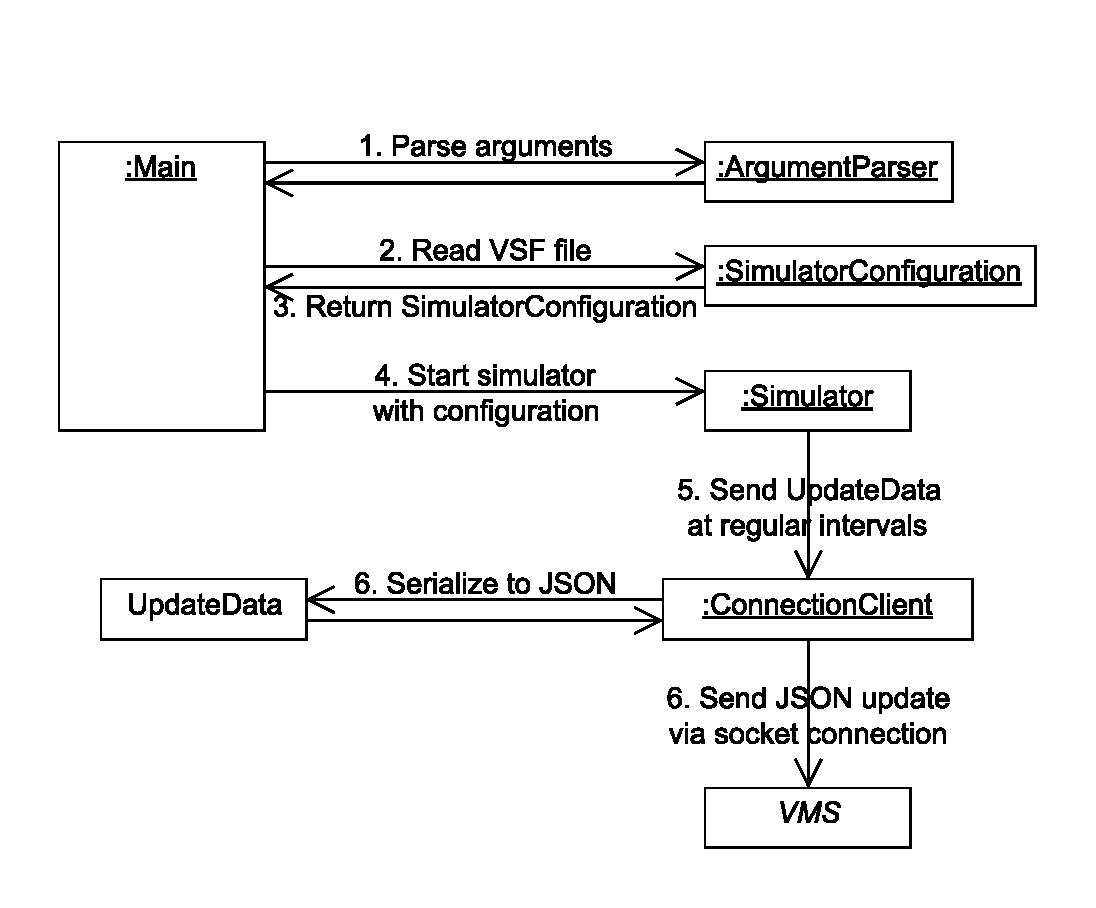
\includegraphics[scale=0.3]{diagrams/simulator-communication-diagram.eps}
\end{figure}

When the program fires up this subsystem will start of and parse the arguments that are given to it. Following that it will read from the vsf file from which it will create a simulatorConfiguration instance. With the configuration created from the vsf file, it will start the simulator.  The simulator will update out of date data to the connection client class at regular intervals. From there it will interact with the updateData class and the VMS subsystem.

\break

\begin{figure}[!htb]
\caption{Class Diagram of the Simulator subsystem}
\centering
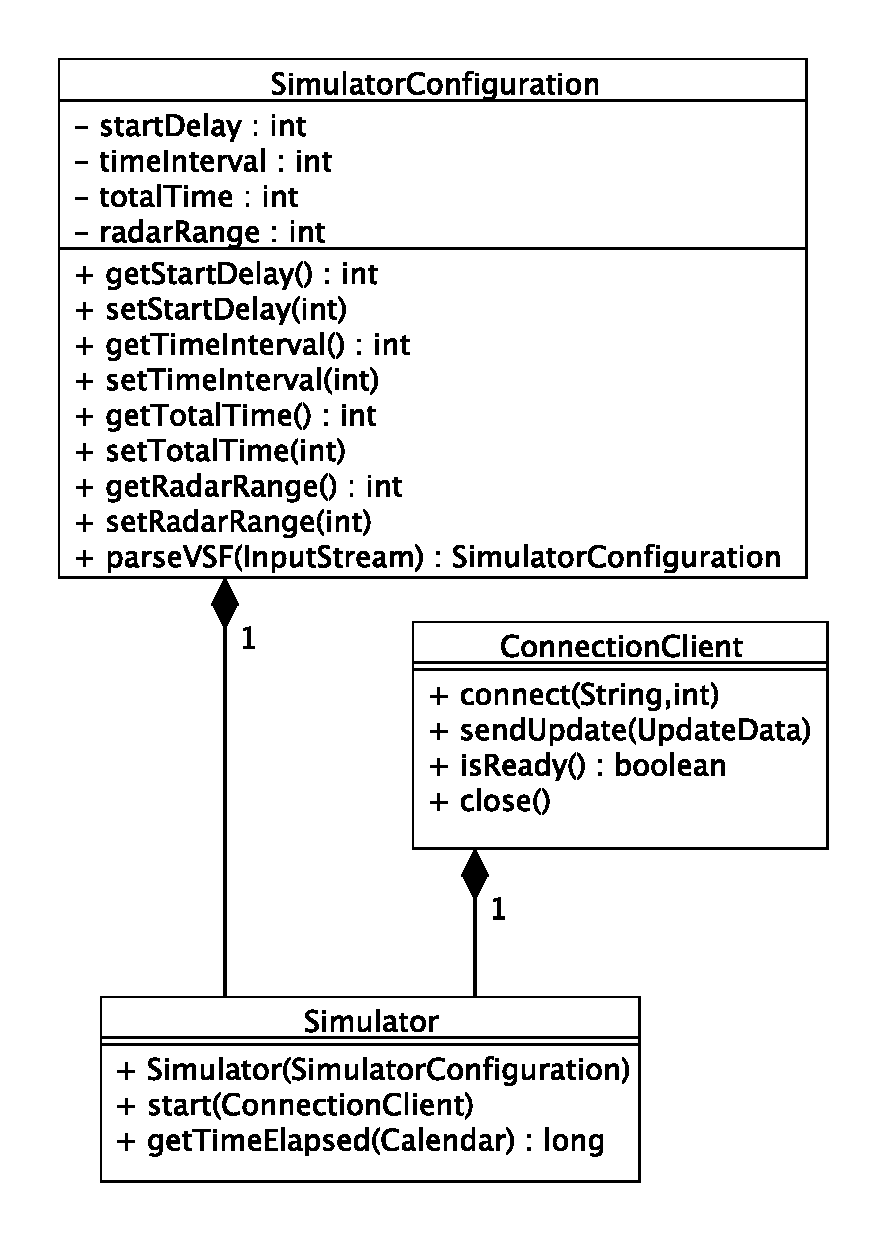
\includegraphics[scale=0.3]{diagrams/simulator-class-diagram.eps}
\end{figure}

These are the classes involved in the configuration process of the creation of the simulator. As stated for figure 1 simulatorConfiguration class will take on a vsf file for it to parse, with that it will ensure that the configuration can set properly. Then from there the simulator will start the connectionClient which enable communication with the vms subsystem.


\begin{figure}[!htb]	
\caption{Class Diagram of VMS subsystem}
\centering
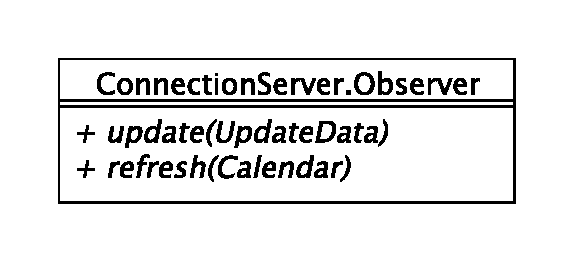
\includegraphics[scale=0.3]{diagrams/vms-class-diagram.eps}
\end{figure}

SOMETHING HERE

\break

\begin{figure}[!htb]
\caption{Communication Diagram of VMS subsystem}
\centering
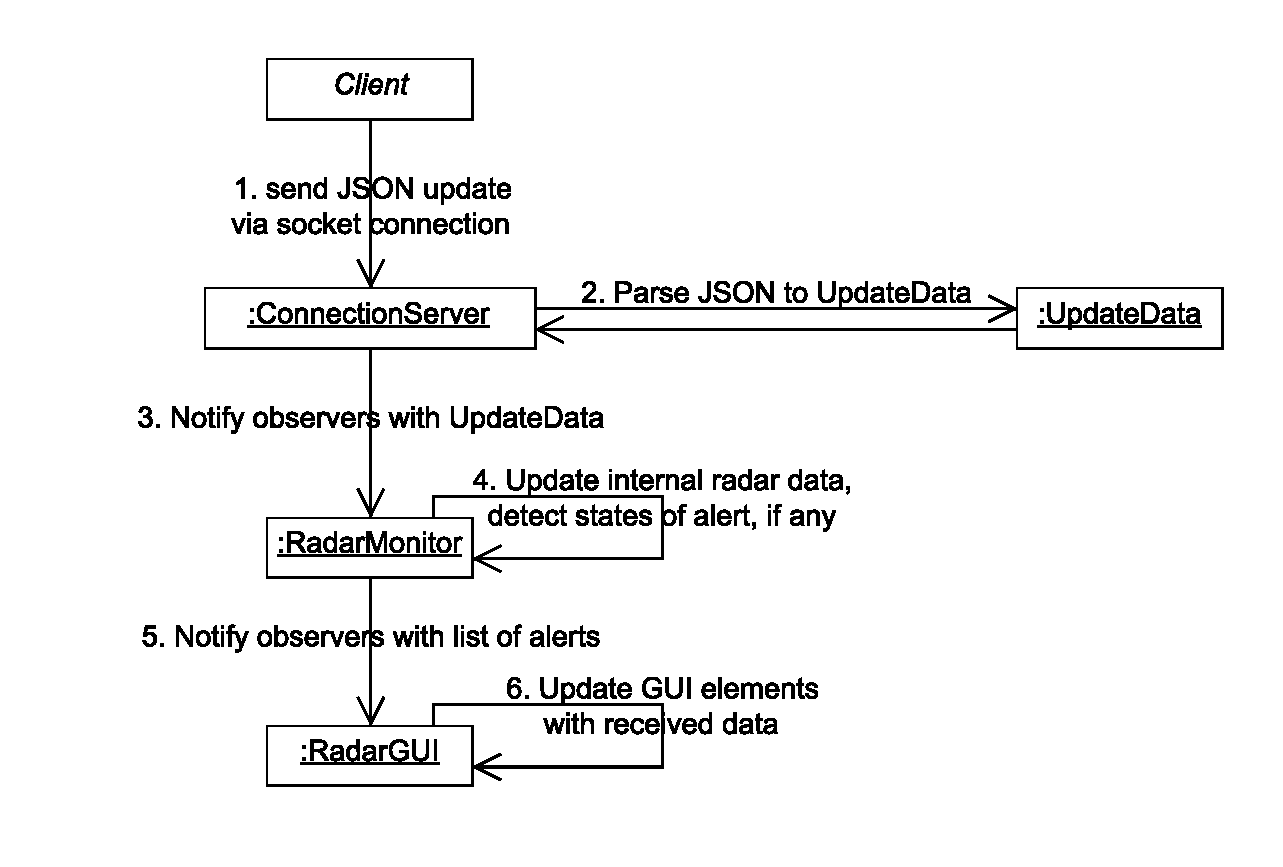
\includegraphics[scale=0.3]{diagrams/vms-communication-diagram.eps}
\end{figure}

When the program starts up, the client will send a JSON update via the socket it will have created to the connection server class. From that point on, it will start communicating with the updateData class for new information. If any data was updated it will notify the observers that the data has been changed, in doing so the radar monitor data will be updated. Inside the radar monitor it will search any data that requires attention (e.g. alerts). If any need attention it will notify the observers (radar gui) with the list of alerts.

\subsubsection{Development View} % Status: Work in Progress

\begin{figure}[!htb]
\caption{Activity Diagram for the Simulator Subsystem}
\centering
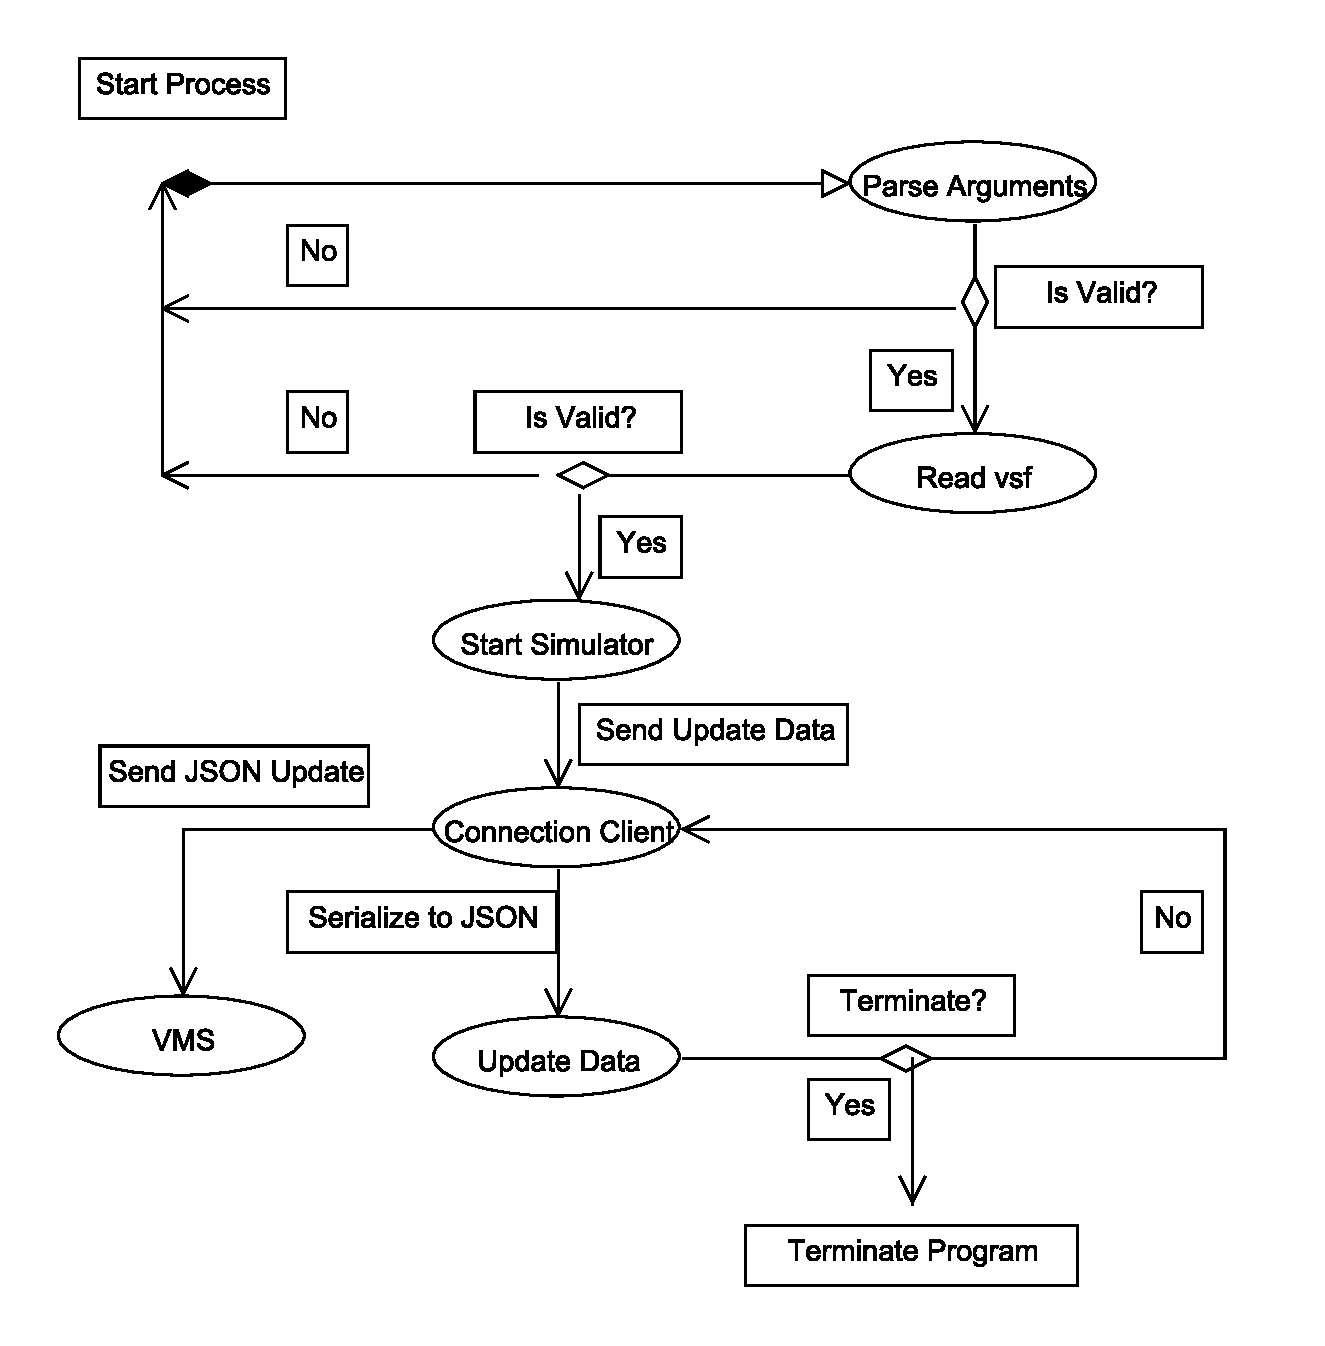
\includegraphics[scale=0.3]{diagrams/simulator-acitivity-diagram.eps}
\end{figure}

Most of the heavy duty is done in the simulator side. It handles multiple steps to ensure the simulator is ready to start running. Even after that it will check regularly if there is new data sent, so it will be able to create updates for the other subsystems.

\break

\begin{figure}[!htb]
\caption{Activity Diagram for the Vessel Monitoring System (VMS) }
\centering
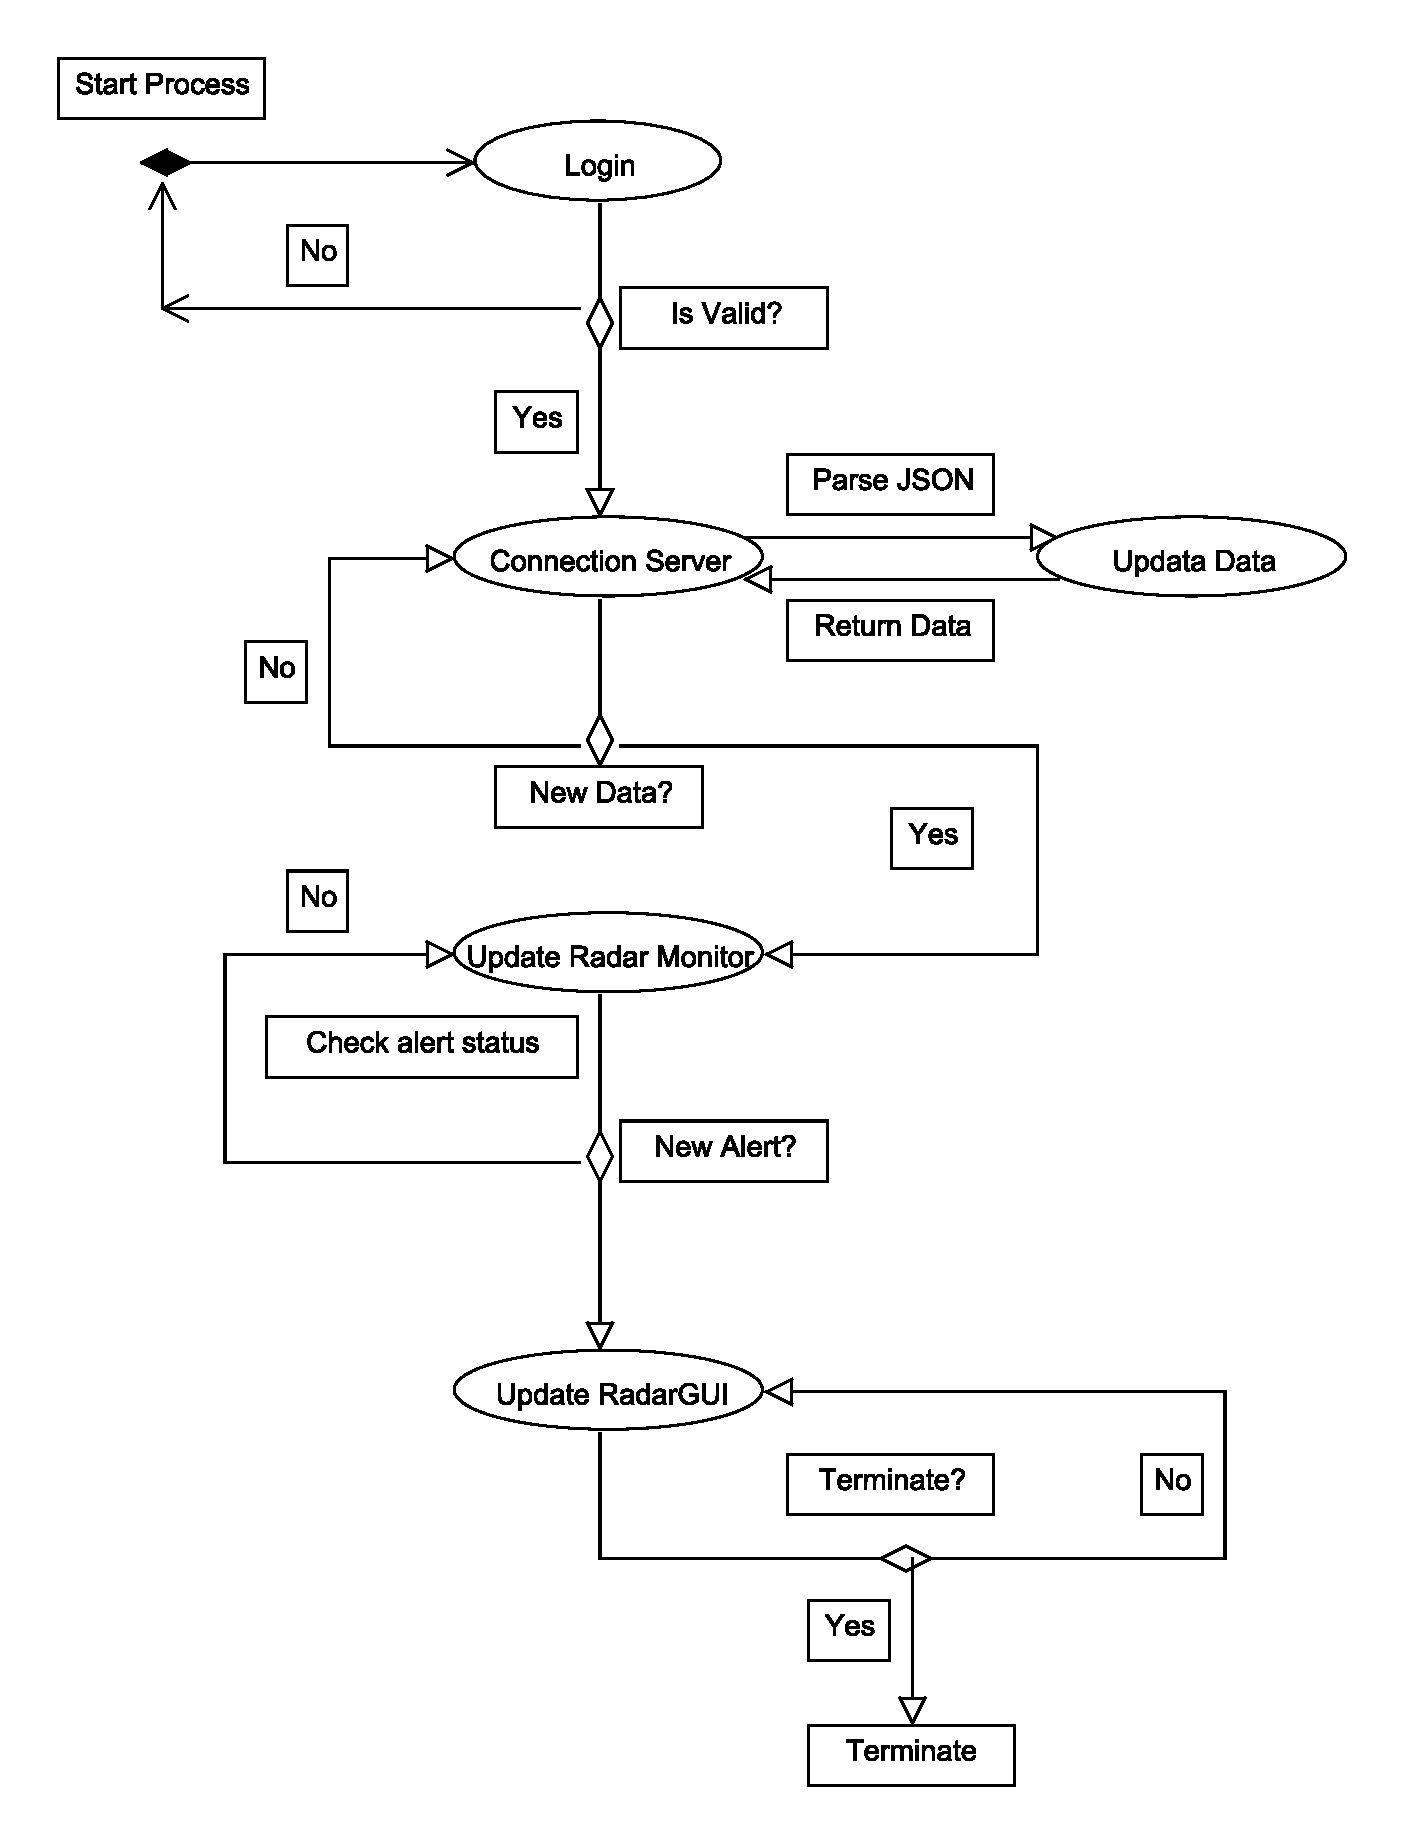
\includegraphics[scale=0.2]{diagrams/vms-activity-diagram.eps}
\end{figure}

The Vessel Monitoring System has the easy part. The only hard job of of the VMS subsystem is parsing the JSON from updataData and from there it will regularly check for new alerts and check if new data is sent to the gui.

\subsection{Subsystem Interfaces Specifications} % Status: See subsubsections

\subsubsection{Simulator subsystem} % Status: Work in Progress

\begin{enumerate}
  \item Parse command-line invocation from user: 
		\newline "./Simulator - -host 192.168.0.1 - -port 1024 - -input filename.vsf"
		\newline Note: - -host, - -port and - -input can be replaced with -h -p -i respectively.
		\newline The arguments must be entered in this order.
  \item In the main method, it will be ensured that the command-line invocation is written as it is above, otherwise the program will exit.
  \item When all cleared, "SimulatorConfiguration.parseVSF(InputStream in)" will return the configuration instance of the simulator.
  \item Any files that are opened at this time will be closed to ensure no unnecessary streams are open.
	\item "ConnectionClient.connect(String host, int port) throws IOException" will take the validated host and port from the command-line and create a new socket for the user.
	\item "Simulator.start(ConnectionClient client)" will take the client instance created in step 5 and use it to start the simulator.	
\end{enumerate}

\subsubsection{VMS subsystem} % Status: Work in Progress

\begin{enumerate}
  \item ConnectionServer.bind(SocketAddress addr) throws IOException
	\item ConnectionServer.start() throws IOException
\end{enumerate}

\break

\section{Detailed Design} % Status: See subsections

\subsection{Subsystems} % Status: See subsubsections

\subsubsection{Detailed Design Diagram} % Status: Work in Progress

\paragraph{Simulator Subsystem} 

\begin{figure}[!htb]
\caption{Simulator Class Diagram}
\centering
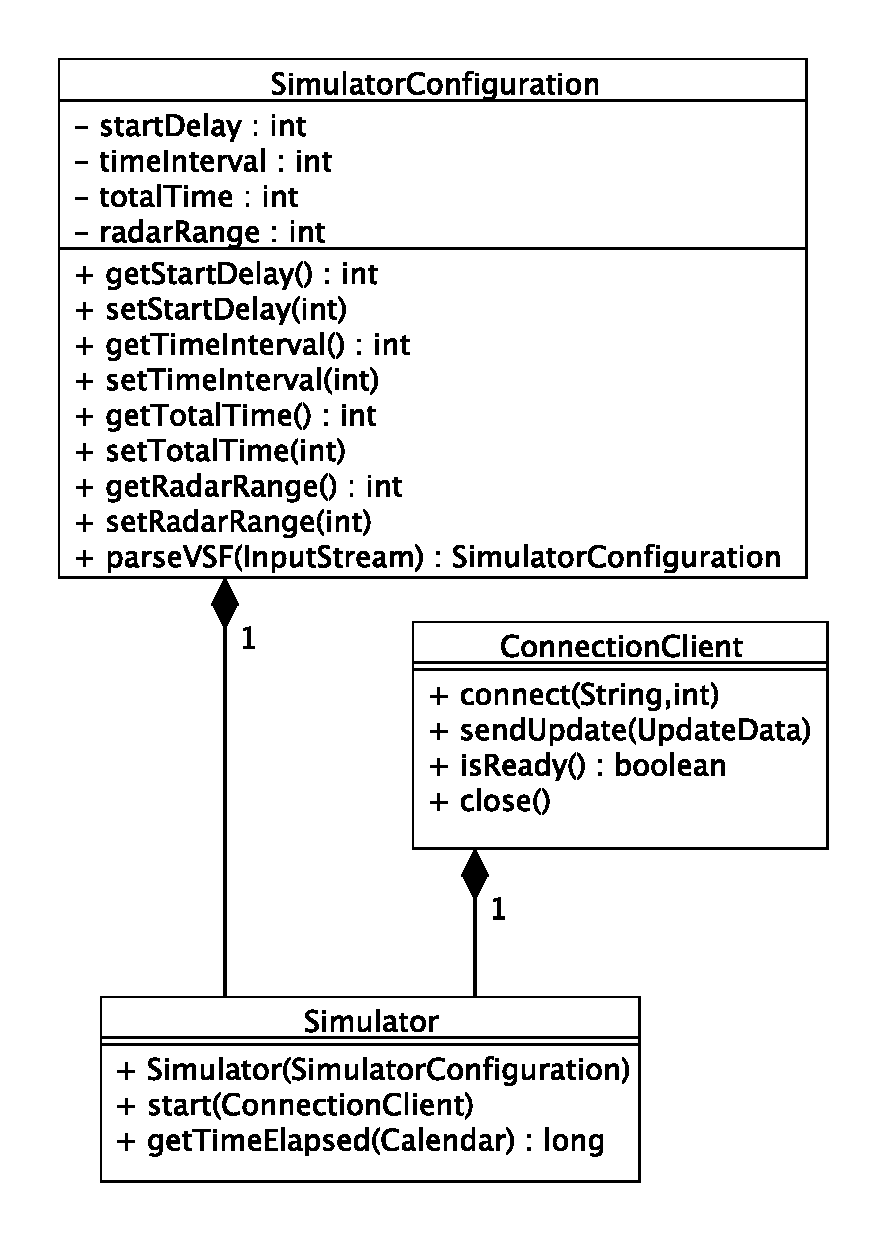
\includegraphics[scale=0.6]{diagrams/simulator-class-diagram.eps}
\end{figure}

The Simulator subsystem is the part of the software that will simulate the actual physical radar and the data it sends to the Vessel Monitoring System (VMS). A .vsf file, which lists the positions and courses of given vessels, as well as various configuration parameters for the VMS, is parsed and interpreted as vessel data by the simulator, which then establishes socket communication with the VMS. The simulator then proceeds to send updated data to the VMS at set intervals, until the pre-defined total time limit expires.

\break

\paragraph{Vessel Monitoring System (VMS) Subsystem}

\begin{figure}[!htb]
\caption{VMS Class Diagram}
\centering
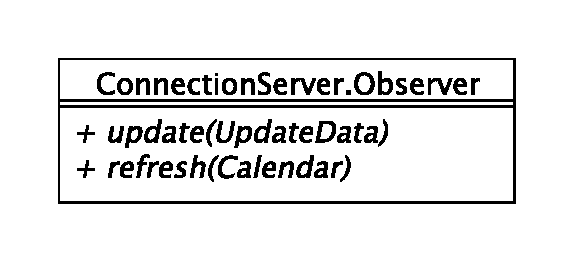
\includegraphics[scale=0.6]{diagrams/vms-class-diagram.eps}
\end{figure}

The Vessel Monitoring System (VMS) subsystem is the part of the software that will receive vessel data from the radar (represented by the Simulator) and interpret this data so that it can be viewed by the user via a graphical interface, and emit high- or low-risk alerts if any two vessels are within a certain range of each other. The VMS accepts socket connections from any number of Simulator instances.

\break

\subsubsection{Unit Descriptions} % Status: Work in Progress

\paragraph{Simulator Subsystem}

\subparagraph{Class SimulatorConfiguration}
The main purpose of this class is to parse the .vsf file and to keep track of the data obtained, as well as registering any modifications to this data.

\vspace{0.5cm}

Attributes:
\begin{enumerate}
    \item private int \_StartDelay
    \item private int \_TimeInterval
    \item private int \_TotalTime
    \item private int \_RadarRange
    \item List\textless Vessel\textgreater \, \_Vessels
\end {enumerate}

\vspace{0.5cm}

Functions:
\begin{enumerate}
	\item private SimulatorConfiguration()
	\item public int getStartDelay()
	\item public void setStartDelay(int)
	\item public int getTimeInterval()
	\item public void setTimeInterval(int)
	\item public int getTotalTime()
	\item public void setTotalTime(int)
	\item public int getRadarRange()
	\item public void setRadarRange(int)
	\item public List\textless Vessel\textgreater  \,getVessels()
	\item public void addVessel(Vessel)
	\item public static SimulatorConfiguration parseVSF(InputStream)
\end{enumerate}

\subparagraph{Class ConnectionClient}
This class is responsible for establishing and managing the socket connection to the VMS, as well as sending all update data via this connection. The sent data is converted to JSON and encoded as Netstring.

\vspace{0.5cm}

Attributes:
\begin{enumerate}
	\item private final int TIMEOUT
    \item private Socket \_Socket
\end {enumerate}

\vspace{0.5cm}

Functions:
\begin{enumerate}
	\item public ConnectionClient()
	\item public void connect(String, int)
	\item public void sendUpdate(UpdateData)
	\item public boolean isReady()
	\item public void close()
\end{enumerate}

\subparagraph{Class Simulator}
This class performs and determines the frequency of data updates and communications to the VMS. Once a connection to the VMS is established, the Simulator creates a thread for a set duration, during which the data from SimulatorConfiguration is updated and sent to VMS through the ConnectionClient at set intervals.

\vspace{0.5cm}

Attributes:
\begin{enumerate}
	\item SimulatorConfiguration \_Configuration
\end {enumerate}

\vspace{0.5cm}

Functions:
\begin{enumerate}
	\item public Simulator(SimulatorConfiguration)
	\item public void start(ConnectionClient)
	\item public long getTimeElapsed(Calendar)
\end{enumerate}

\vspace{0.25cm}

\paragraph{Vessel Monitoring System (VMS) Subsystem}

\subparagraph{Class ConnectionServer}
The purpose of this class is to accept connections established by one or more radars, and receive the transmitted data. In addition, observers may be registered so that they will be notified of every incoming data update.

\vspace{0.5cm}

Attributes:
\begin{enumerate}
	\item private static long DEFAULT\_REFRESH
    \item private boolean \_Continue
    \item private long \_RefreshTime
    \item private Selector \_Selector
    \item private ServerSocketChannel \_Channel
    \item private List\textless Observer\textgreater \,\_Observers
\end {enumerate}

\vspace{0.5cm}

Functions:
\begin{enumerate}
	\item public ConnectionServer()
	\item public void setMinimumRefresh(long)
	\item public long getMinimumRefresh()
	\item public void registerObserver(Observer)
	\item public void unregisterObserver(Observer)
	\item public void refreshObservers(Calendar)
	\item public void updateObservers(UpdateData)
	\item public void bind(SocketAddress)
	\item public void setRadarRange(int)
	\item public List\textless Vessel\textgreater \,getVessels()
	\item public void addVessel(Vessel)
	\item public static SimulatorConfiguration parseVSF(InputStream)
\end{enumerate}

\subparagraph{Class RadarMonitor (implements ConnectionServer.Observer)} % Status: To be done

\subparagraph{Class RadarDisplay (implements RadarMonitor.Observer)} % Status: To be done

\subparagraph{Class Vessel}
This class represents a vessel and all of its relevant characteristics.

\vspace{0.5cm}

Attributes:
\begin{enumerate}
	\item private VesselType type
    \item private String id
    \item private Course course
    \item private Coord coords
    \item private Calendar lastTimestamp
\end {enumerate}

\vspace{0.5cm}

Functions:
\begin{enumerate}
	\item public Vessel(String, VesselType)
	\item public String getId()
	\item public VesselType getType()
	\item public Coord getCoord(Calendar)
	\item public Course getCourse(Calendar)
	\item public Calendar getLastTimestamp()
	\item public void update(Coord, Course, Calendar)
	\item public void update(UpdateData)
	\item public UpdateData getUpdateData(Calendar)
\end{enumerate}


\section{Dynamic Design Scenarios} % Status: To be done

[Give a full dynamic design of two substantial use cases including system sequence diagrams operational contracts, and sequence diagrams. Units and subsystems depicted here must be compatible with the descriptions provided in section 2 and 3.]

\section{Revised Cost Estimation} % Status: Work in Progress

[Provide a revised estimated cost, as well as the basis for those estimates, and the points and circumstances in the project when re-estimation might occur.
Evaluate the cost of production of each artifact, as described in the previous section, and then adding up the numbers.]

\vspace{0.5cm}

\emph{Simulator program}: x hours of coding. Due date: August 1st, 2013.

\emph{VMS program}: x hours of coding. Due date: August 1st, 2013.

\emph{Graphical User Interface}: 5 hours of coding. Due date: August 7th, 2013.

\emph{Unit test suite}: 12 hours of implementation. Due date: August 9th, 2013.

\emph{Final integration}: 6 hours of implementation. Due date: August 12th, 2013.

\end{document}


